\chapter{Analýza}

\section{Monitorovanie vibrácií a šoku}
Vibrácie sú periodickým kmitaním hmoty okolo rovnovážnej polohy vznikajúce excitáciou látky, ktorej je dodaná potenciálna energia, a zo
zákona zachovania energie je následne premieňaná na kinetickú energiu. V realite dochádza pôsobením trenia k útlmu voľného oscilačného
pohybu s časom  a pohybová energia sa uvoľňuje v podobe tepelnej alebo akustickej emisie do okolitého prostredia. Častejšie ako presné
harmonické kmity sú pozorované náhodné vibrácie, ktorých vývoj nevieme dopredu predvídať. Naproti tomu šok, alebo aj prechodový jav, je
náhle uvoľnenie kinetickej energie krátkeho trvania oproti prirodzenej oscilácii systému.

Význam a dôležitosť sledovania vibrácií spočíva v ich výskyte u každého mechanického zariadenia a je zapríčinená pohybom jednotlivých
súčiastok a trením v ložiskách. Ich nadmerná prítomnosť býva spôsobená opotrebením dielov stroja alebo nevyvážením rotačných častí,
zakliesňovaním ozubených kolies, ako dôsledkoch iných technických defektov. V prevažnej väčšine prípadov ide o nežiaduci jav nakoľko
zakladá zníženiu účinnosti so zvýšením hlučnosti ako vedľajšiemu produktu.

Ďalšou oblasťou hojnej prítomnosti vibrácií je preprava osôb alebo tovaru cestnými a železničnými dopravnými prostriedkami, kde sú
zapríčinené nerovnosťami povrchu vozovky alebo koľaje v bode styku s kolesami vozidla. Na zvýšenie ovládateľnosti vozidla a komfortu
pasažierov sú kabíny odpružené od kolies tlmičmi. Lietadlá sú zasa pod vplyvom trenia vzduchu s trupom a krídlami konštrukcie, ktoré je
ďalej zosilnené vzdušnými prúdmi a turbulenciami.

Druhým významným faktorom podieľajúci sa na tvorbe vibrácii je aparát, ktorý uvádza vozidlo do pohybu alebo zastavuje, čiže hnací
najčastejšie spaľovací, dieselový alebo elektrický motor a brzdový systém. Jedná sa najmä o vplyv pohybu piestov, alebo rotora u
elektrických vozidiel, a prenosu otáčavého pohybu motora cez oje hriadeľa na nápravy. ABS brzdový systém prítomný pri väčšine
automobilov zabraňujú šmyku striedavým zomknutím a uvoľňovaním brzdových kotúčov, čo má tiež vplyv na podmienky počas jazdy.

Detekciou nežiaducich vibrácií v preprave sa dokáže zabezpečiť aj bezpečnosť pasažierov včasnou výmenou súčiastky, ktorá by ovplyvnila
prevádzkyschopnosť v kritických momentoch. Ich eliminácia dokáže predísť nenávratnému poškodeniu krehkých materiálov alebo
znehodnoteniu reaktívnych substancií, či dokonca ich aktivácii v prípade výbušnín a pyrotechniky.

V neposlednom rade sú vibrácie súčasťou potenciálne nebezpečných prírodných úkazov a ich správna identifikácia má za následok varovania
pre preventívnu evakuáciu obyvateľstva v oblasti, ktoré bude zasiahnutá zemetrasením, či erupciou sopky vedúcimi k ohrozenia zdravia
osôb a poškodenia majetku.

\subsection{Meranie fyzikálnej veličiny akcelerácie}
Pohyb mechanického systému vystaveného vonkajším silám sa nazýva odozva, ktorej správanie opisuje zjednodušený model s jedným stupňom
voľnosti (1DOF) kmitajúceho telesa s pružinou a tlmičom \cite{vibrations-shock}.

\begin{figure}[h]
	\centering
	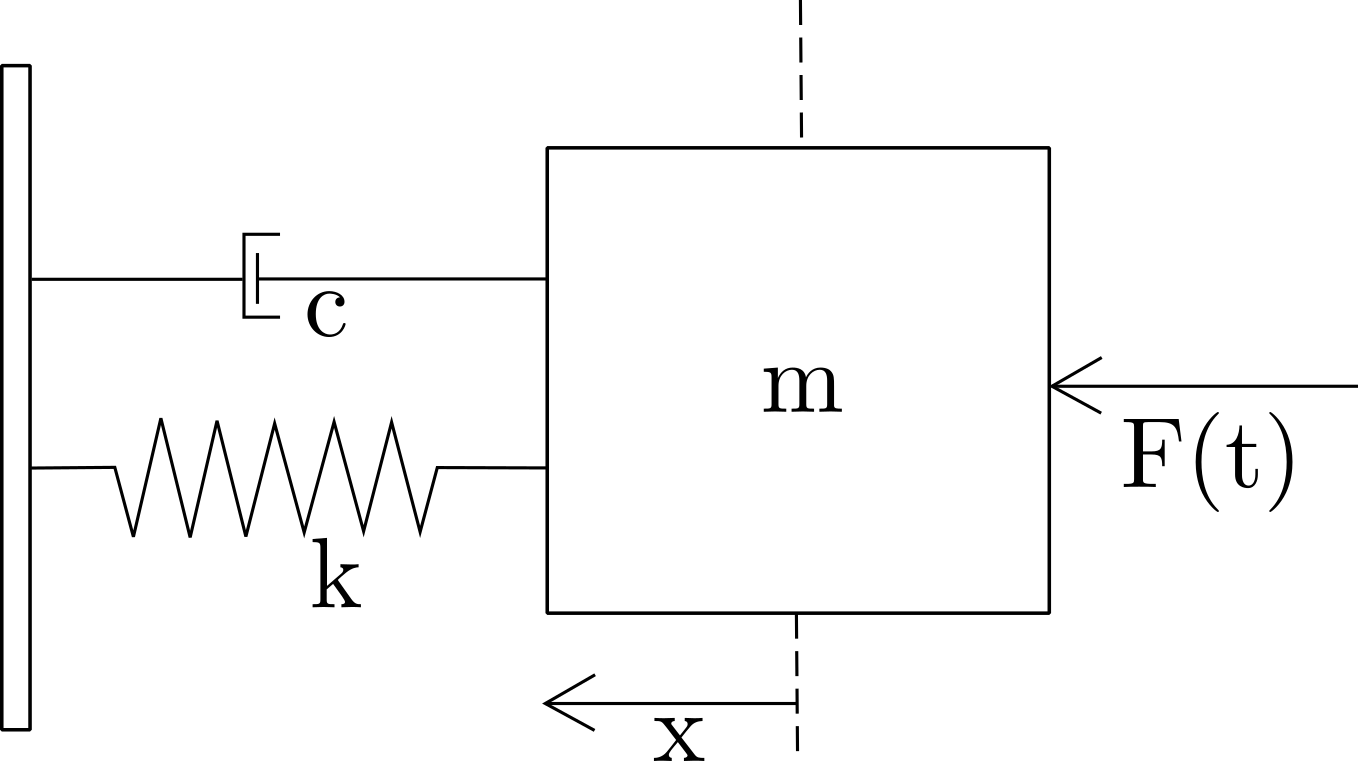
\includegraphics[width=0.7\textwidth]{figures/mass-spring-damper-model.png}
	\caption{Model oscilujúceho systému s pružinou a tlmičom}
\end{figure}

Pri pôsobení vonkajšej sily $F$ na hmotu upevnenú na pružine vznikajú nútené vibrácie, ktoré ju vychyľujú z rovnovážnej polohy. Uvedená sila je charakterizovaná druhým Newtonovým zákonom v tvare $F = ma$, kde $m$ je hmotnosť telesa a $a$ predstavuje zrýchlenie. V protismere pôsobí sila vyvolaná pružinou $F_s = -kx$ a tlmiacim členom $F_d = -cv$, kde $k$ je tuhosť pružiny ovplynená jej konštrukciou, $c$ je tlmiaci koeficient, $x$ je vychýlenie z rovnovážneho stavu, a $v$ rýchlosť vychýlenia. 

Fyzickým obmedzením  telesa, ktorým je viazaný na pevnú podložku dochádza pri zanedbaní deformácie k takmer zaručenému návratu do rovnovážnej polohy a to nám umožňuje merať intenzitu vibrácií cez zrýchlenie ťažidla. Výslednú silu v jednom smere získame sčítaním síl podieľajúcich sa na dynamike telesa.
\begin{ceqn}\begin{align}
 	F(t) = ma - cv - kx
\end{align}\end{ceqn}
Pri použití trojosového akcelerometra, kedy sú evidované všetky tri priestorové súradnice časovo-premennej akcelerácie dostávame
nasledujúcu rovnicu vo vektorovom tvare:
\begin{ceqn}\begin{align}
   \vec{a}(t) = \frac{\vec{F}(t)}{m}
\end{align}\end{ceqn}
Magnitúda akcelerácie s troma súradnicami je daná $L_2$ normou vektora $\vec{a} = (a_x, a_y, a_z)$:
\begin{ceqn}\begin{align}
   |a| = \sqrt{a_x^2 + a_y^2 + a_z^2}
\end{align}\end{ceqn}

\subsection{MEMS kapacitný akcelerometer}
Bežné inerciálne senzory na meranie zrýchlenia priamočiareho, ale aj rotačného pohybu (gyroskop), sa vyrábajú technológiou
\emph{MEMS – mikromechanický systém}, kedy je celé zariadenie vrátane všetkých mechanických súčastí umiestnené na kremík procesom
mikrovýroby vo viacerých vrstvách. Sila spôsobujúca zrýchlenie je potom meraná vychýlením vstavanej odpruženej hmoty vzhľadom
na pevné elektródy, ktoré môžu byť usporiadané jednostranne alebo ako diferenčný pár \cite{mdof-mems-accelerometers}.

\begin{figure}[h]
	\centering
	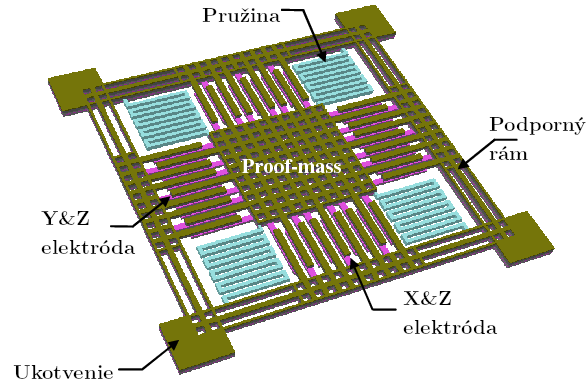
\includegraphics[width=0.8\textwidth]{figures/mems-accelerometer.png}
	\caption{Mikroštruktúra 3DOF MEMS kapacitného akcelerometra \cite{microstructure-mems}}
	\label{fig:mems}
\end{figure}

Pri diferenčnom páre spôsobí pohyb doštičky ťažidla medzi elektródami zmenu kapacít a ich rozdielom je možné zistiť aplikovanú silu a
cez uvedený vzťah zrýchlenie. Na zvýšenie celkovej kapacity sa používa viacero párov elektród zapojených paralelne. Pred prevodom na
číslicový signál musí napäťová úroveň zo senzora prejsť úpravou zahŕňajúcou nábojovocitlivý predzosilňovač, osovú demoduláciu a anti-
aliasingové filtrovanie. 

Viacosové akcelerometre vyžadujú viaceré opísané štruktúry orientované kolmo na seba, podľa obr. \ref{fig:mems}, s ohľadom na počet 
vyžadovaných stupňov voľnosti, pričom v skutočných senzoroch vždy existuje aspoň minimálna závislosť medzi osami rádovo najviac v 
jednotkách percent. Teplota ovplyvňuje citlivosť MEMS akcelerometrov len nepatrne v stotinách percenta na stupeň Celzia.

Akcelerometre sa odlišujú v niekoľkých dôležitých vlastnostiach, ktoré zvyknú byť nastaviteľné vo výrobcom stanovenom rozsahu
prípustných hodnôt s príslušnými toleranciami \cite{accelerometer-mechanics}.

\emph{Citlivosť} stanovuje najmenšiu rozlíšiteľnú zmenu v odčítanom napätí ku zmene externého pohybu respektíve zrýchlenia.
Uvádza sa v jednotkách \emph{mV/g} (milivolt na tiažové zrýchlenie) pri analógovom výstupe, alebo \emph{mg/LSB} (mili-g
na najmenej významový bit). pri senzoroch so vstavaným analógovo-digitálnym prevodníkom. Jednotka \emph{mg/LSB} vyjadruje
o koľko sa zmení zrýchlenie keď zvýšime alebo ponížime binárne číslo na výstupe o jedna. Niekedy sa namiesto
citlivosti uvádza mierka pre presnosť ako prevrátená hodnota citlivosti v \emph{LSB/g}. Tiažové zrýchlenie $g$ sa mierne líši podľa
zemepisnej šírke, ale stanovený prepočet na jednotky SI je $1 g = 9.80665\,m/s^2$
\footnote{\url{https://physics.nist.gov/cgi-bin/cuu/Value?gn|search_for=acceleration}}.

\emph{Dynamický rozsah} sa uvádza v tiažovom  zrýchlení $g$. Hovorí o najmenšej a najväčšej rozlíšiteľnej hodnote zrýchlenia nad
úrovňou ktorej už dochádza k skresleniu signálu orezaním špičiek. S nevyhnutnými drobnými nepresnosťami výroby mikromechaniky je tzv.
\emph{zero-g napätie} popisujúce odchýlku skutočného od ideálneho výstupu, keď na sústavu nepôsobí žiadne zrýchlenie. Za ideálnych
okolností bez pohybu na vodorovnom povrchu namerajú osi $x$ a $y$ zrýchlenie $0g$, zatiaľčo na $z$ pôsobí $1g$. Očakávaním je nulová
hodnota výstupného napätia a tým aj výstupného registra.

\emph{Šírka pásma} senzora v \emph{Hz} predurčuje rozsah frekvencie vibrácií, ktoré je možné zachytiť. Podmienená je zvolenou
početnosťou  čítania akcelerácie za sekundu, čiže vzorkovacou frekvenciou. Stanovuje sa tiež nastaviteľným parameterom \emph{ODR}
(Output Data Rate) - výstupný dátový tok, pričom šírka pásma je spravidla polovicou ODR. Menej uvádzanou vlastnosťou býva 
\emph{frekvenčná odozva} senzora, ktorá určuje o koľko sa v rámci tolerancie odlišuje skutočná 
citlivosť od referenčnej pre zodpovedajúcu frekvenciu vibrácii. 

Na meranie zrýchlenia má nevyhnutný vplyv šum zapríčinený Brownovým  pohybom a nedokonalosťou skutočných materiálov v štruktúre 
akcelerometra. Intenzita šumu rastie inverznou odmocninou so šírkou pásma, čiže s častejším meraním získavame menšiu presnosť. Pri 
dostatočnom odstupe signálu od šumu, $SNR = P_{signal} / P_{šum}$, umožňuje hardvér akcelerometra vzorkovať amplitúdy až nad stanovený 
prah generovaním prerušenia, čím sa dokáže efektívne zbaviť nevýznamných fluktuácií.

\subsection{Analógovo-digitálny prevodník}
Spojitá napäťová úroveň transformuje analógovo-digitálny (A/D) prevodník pre spracovanie digitálnym systémom do množiny diskrétnych
hodnôt. Vstupný signál najprv prechádza fázou vzorkovania, kedy sa vzorky zaznamenávajú v pravidelných intervaloch. Počet vzoriek
odčítaných za sekundu je vyjadrený vzorkovacou frekvenciou $f_s$ v $Hz$. Časový rozdiel medzi vzorkami, nazývaný perióda vzorkovania,
je prevrátenou hodnotou vzorkovacej frekvencie $T_s = \frac{1}{f_s}$. Pre presnú rekonštrukciu pásmovo obmedzeného signálu v hraniciach
$[-f_{max}; f_{max}]$ je nevyhnuté podľa \emph{Nyquist-Shannonovej vety} o vzorkovaní, aby vzorkovacia frekvencia bola najmenej 
dvojnásobkom maximálnej frekvencie snímaného signálu.
\begin{ceqn}\begin{align}
   f_s \geq 2 \cdot f_{max}
\end{align}\end{ceqn}

Každej vzorke je následne v procese kvantovania priradená diskrétna hodnota s konečným počtom $n$ bitov, ktorá je najbližšia možná ku
skutočnej hladine analógového vstupu. Dochádza pritom k istému zaokrúhľovaniu z dôvodu nepresnosti vyjadrenia spojitej domény amplitúd
diskrétnym číslom. Tento jav označujeme ako kvantizačný šum, ktorý je najviac polovicou z maximálnej rozlíšiteľnej zmeny signálu a
trpia nim všetky existujúce A/D prevodníky.

\begin{figure}[h]
	\centering
	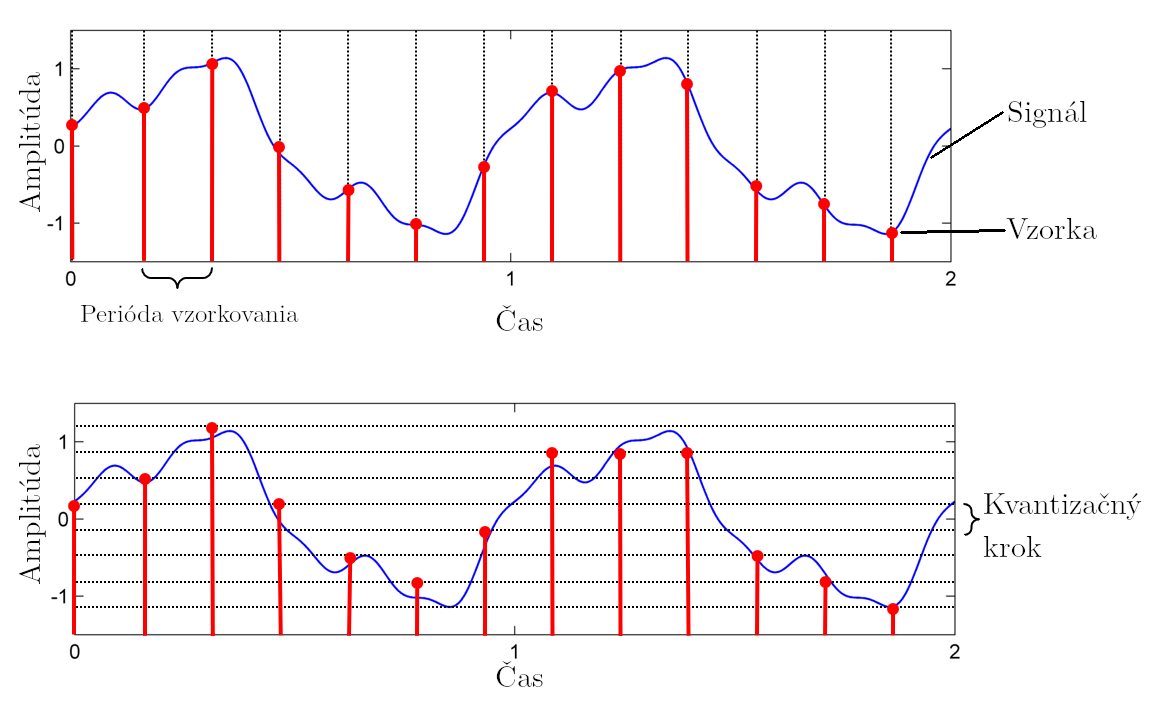
\includegraphics[width=0.8\textwidth]{figures/analog-to-digital-conversion.png}
	\caption{Digitalizácia signálu v analógovo-digitálnom prevodníku \cite{music-processing}}
\end{figure}

Prevodníky integrované priamo s inerciálnymi jednotkami sa vyhotovujú v rozlíšeniach 12, 16 alebo 20 bitov. Umožňujú tak pripojiť
akcelerometer rovno na sérové zbernice \emph{SPI} alebo \emph{I2C}. Všeobecne platí, že pri $n$ bitoch je k dispozícii $2^n$ rozličných
čísel. Kódovaním v dvojkovom doplnku pre zachytenie záporných hodnôt sa uvažuje s intervalom $[-2^\frac{n}{2}; 2^\frac{n}{2} - 1]$.

Napríklad pri 12-bitovom A/D prevodníku s referenčným napätím $3.3V$ je teoreticky najmenšia rozlíšiteľná zmena na najmenej významový
bit $3.3V / 2^{12} = 0.81 mV$. Ak je rozhranie senzora priamo vybavené analógovým výstupom nič nebráni v použití presnejšieho
prevodníka, napriek tomu najmenší merateľný dielik je zdola stále ohraničený citlivosťou akcelerometra.

Číslicová hodnota v dvojkovom doplnku získanú konverziou $\hat{x}$ je prepočítaná na
štandardné fyzikálne jednotky pre zrýchlenie, $a$ v $m/s^2$). $R$ prestavuje nastavený dynamický rozsah v jednotkách $g$ a $n$
je počet bitov A/D prevodníka.
\begin{ceqn}\begin{align}
   a = \hat{x} \cdot ((R \cdot g) / 2^{n / 2})
\end{align}\end{ceqn}

Na základe už zmieneného ohľadom vlastností MEMS akcelerometrov, presnejší prevod dosiahneme zužitkovaním deklarovanej citlivosti
senzora pri danom dynamickom rozsahu $S_R$ udávaného v $mg/LSB$.
\begin{ceqn}\begin{align}
   a = \hat{x} \cdot (S_R \cdot g) / 1000
\end{align}\end{ceqn}

\subsection{Vlastnosti bežných akcelerometrov}
Na ilustráciu uvádzame parametre zvolených najrozšírenejších typov akcelerometrov. Akcelerometer LSM9DS1 \cite{lsm9ds1} umožňuje cez
zbernicu SPI alebo I2C zvoliť zo štyroch dynamických rozsahov, pričom každé rozpätie sa vyznačuje svojou citlivosťou. Zvolením menšieho
dynamického rozsahu zvýšime citlivosť. LSM9DS1 funguje pri rozsahoch $\pm2$g, $\pm4$g a $\pm8$g a $\pm16$g, postupne s citlivosťami
$0.061$ mg/LSB, $0.122$ mg/LSB, $0.244$ mg/LSB, $0.732$ mg/LSB. Výstupný dátový tok (ODR) je možné nastaviť na $10$Hz, $50$Hz,
$119$Hz, $238$Hz, $476$Hz a najvyššie na $952$ Hz. Navzorkované hodnoty sú ukladané do 16-bitového výstupného registra v
dvojkovom doplnku.

Nízkoenergetický 3DOF MEMS akcelerometer ADXL362 \cite{adxl362} so spotrebou $2\,\mu A$ pri $100$Hz disponuje
rozsahmi $\pm2$g, $\pm4$g a $\pm8$g s citlivosťami $1$, $2$ a $4$ mg/LSB. Dostupné vzorkovacie frekvencie 12-bitového A/D prevodníka sú
$12.5 - 400$Hz v 8 krokoch vždy po násobkoch predošlého kroku. Pre rýchlejšie čítanie pri nižšom rozlíšení dokáže senzor zakódovať dáta
do 8-bitového registra.

Vyrábajú sa tiež akcelerometre s väčšími dynamickými rozsahmi a nízkym šumom, ide napríklad o ADXL356 a ADXL357 \cite{adxl357} so
škálami $\pm 10$g, $\pm 20$g a $\pm 40$g s citlivosťou $0,019$ mg/LSB po $0,078$ mg/LSB a rozlíšením A/D prevodníka 20 bitov pri
ODR $4 - 4000$Hz. ADXL357 ponúka priamo analógové výstupy s citlivosťou $20 - 80$ mV/g pri napájaní $3.3$ V.

\subsection{Odvodzovanie rýchlosti a dráhy zo zrýchlenia}
Meranie akcelerácie umožňuje zároveň nepriamo získať ďalšie údaje o pohybe celkovom v priestore ako aj spôsobenom vibráciami.
Zrýchlenie $\vec{a}$ je definované ako časová zmena rýchlosti $\vec{v}$, zatiaľčo rýchlosť je časovou zmenou polohy $\vec{r}$. Na
pozorovanie prechodových javov alebo na vyjadrenie miery plynulosti pohybu slúži ryv $\vec{j}$, ktorý je časovou zmenou akcelerácie.
Pokiaľ nie sú známe počiatočné podmienky v okamihu začiatku snímania akcelerácie, budú hodnoty veličín relatívne vzhľadom na
štart záznamu. Kinematika v diskrétnom čase je potom opísaná nasledujúci rovnicami, kde $\Delta$ je operátor diferencie
$\Delta t = t(i) - t(i-1)$:

\begin{ceqn}\begin{align}
   \vec{v} = \frac{\Delta \vec{r}}{\Delta t}; \;\;
   \vec{a} = \frac{\Delta \vec{v}}{\Delta t}; \;\;
   \vec{j} = \frac{\Delta \vec{a}}{\Delta t}
\end{align}\end{ceqn}

Vyjadrenie neznámych premenných vzhľadom na akceleráciu spočíva v prenásobení rovníc členom $\Delta t$, čím sa získajú
vzťahy pre okamžitú dráhu a okamžitú rýchlosť. Spočítaním čiastkových okamžitých rýchlostí na intervale dostaneme celkovú rýchlosť a
rovnaký úsudok platí pre polohu. V spojitom čase, keď by vzorkovacia perióda bola nekonečne krátka, dochádza naproti tomu k
integrovaniu funkcie akcelerácie. Dostávame, že rýchlosť je integrálom zrýchlenia a poloha je dvojným integrálom zrýchlenia:

\begin{ceqn}\begin{align}
   \vec{v}(t) = \vec{a_0} + \int{\vec{a}(t)\,\mathrm{dt}} \\
   \vec{r}(t) = \vec{r_0} + \vec{v_0}t + \iint{\vec{a}(t)\,\mathrm{dt}}
\end{align}\end{ceqn}

\subsection{Numerická kvadratúra}
Približný výpočet určitého integrálu funkcie akcelerácie je založený na geometrickej interpretácii integrálu ako plochy pod krivkou.
Hovoríme vtedy o probléme numerickej kvadratúry, ktorý navrhuje nahradiť pôvodný integrand interpolačným polynómom 
\cite{numerical-mathematics}. Rád polynómu $n$ implicitne stanoví priebeh funkcie medzi ekvidištantnými vzorkami a 
má dopad na presnosť aproximácie. Najčastejšie sa používajú konštantný ($n = 0$), lineárny ($n = 1$) alebo kvadratický ($n = 2$) 
polynóm, podľa toho rozlišujeme obdĺžnikové pravidlo (vzorec \ref{eq:midpoint-rule}),
lichobežníkové pravidlo (vzorec \ref{eq:trapezodial-rule}) a Simpsonovo pravidlo (vzorec \ref{eq:simpson-rule}).

\begin{ceqn}
\begin{align}
   v(t_i) &= T_s \cdot a\left(\frac{t_i + t_{i-1}}{2}\right)  \label{eq:midpoint-rule} \\
   v(t_i) &= \frac{T_s}{2} \cdot [a(t_i) + a(t_{i-1})]		\label{eq:trapezodial-rule} \\
   v(t_i) &= \frac{T_s}{3} \cdot [a(t_{2i}) + 4a(t_{2i - 1}) + a(t_{2i - 2})] \label{eq:simpson-rule}
\end{align}
\end{ceqn}

Pri \emph{obdĺžníkovom pravidle} (obr. \ref{fig:midpoint-rule}) nepripúšťame zmenu hodnoty zrýchlenia medzi vzorkami a okamžitú 
rýchlosť, čiže plochu, odhadneme ako dĺžku intervalu vzorkovania vynásobenú priemerom výšok dvoch následných pozorovaní. Interpolačný 
polynóm je konštantná funkcia. \emph{Lichobežníkové pravidlo} (obr. \ref{fig:trapezodial-rule}) uvažuje s lineárnou zmenou veličiny 
medzi meraniami, preto interpoluje priamkou.\emph{Simpsonovo pravidlo} (obr. \ref{fig:simpson-rule}) sa snaží o ešte tesnejší odhad s 
využitím kvadratickej funkcie. Každé kvadratúrne pravidlo sa síce vyznačuje presne vyčísliteľnou chybovosťou, ale k tomu je nevyhnutné 
poznať analytické vyjadrenie vibrácií, čo dáva realistický odhad len pri čisto periodických kmitoch.

\begin{figure}[h]
\centering
\begin{subfigure}[b]{0.32\textwidth}
    \centering
    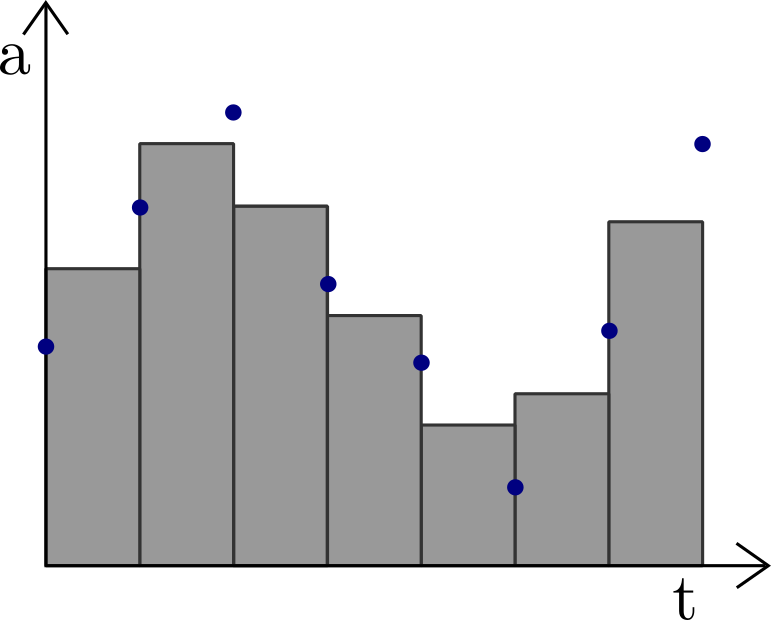
\includegraphics[width=\textwidth]{figures/rectangular-rule.png}
    \caption{Obdĺžníkové}
    \label{fig:midpoint-rule}
\end{subfigure}
\hfill
\begin{subfigure}[b]{0.32\textwidth}
    \centering
    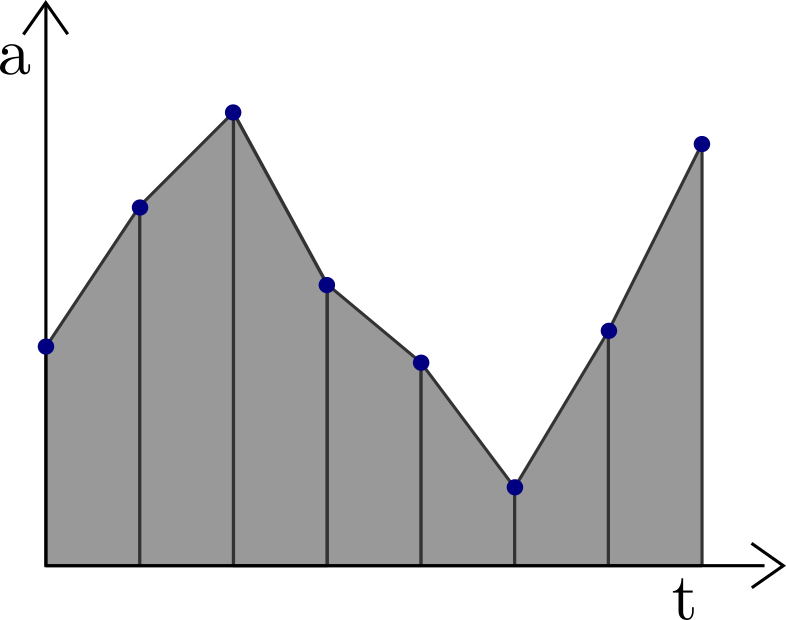
\includegraphics[width=\textwidth]{figures/trapezoidal-rule.png}
    \caption{Lichobežníkové}
    \label{fig:trapezodial-rule}
\end{subfigure}
\hfill
\begin{subfigure}[b]{0.32\textwidth}
    \centering
    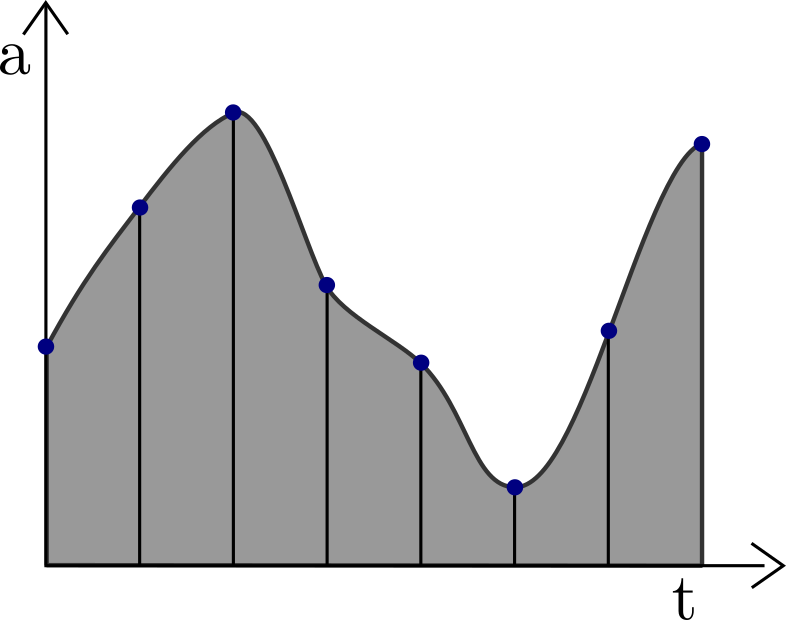
\includegraphics[width=\textwidth]{figures/simpson-rule.png}
    \caption{Simpsonovo}
    \label{fig:simpson-rule}
\end{subfigure}
\caption{Porovnanie pravidiel numerickej integrácie}
\end{figure}

Priama integrácia zašumeného signálu zrýchlenia vedie k neskutočnému driftu, ktorý je ešte zvýraznený dvojitou integráciou pri
odvodzovaní relatívneho posunutia. Dochádza k zosilneniu nízkych a potlačeniu vyšších frekvencií, čím sa začne dominovať neexistujúci
trend vo výstupných dátach. Očakávané oscilujúce správanie vychýlenia u vibrácií so zväčšujúcim sa počtom sčítancov pri rekurentnom
výpočte zaniká. Na zlepšenie stability integrátora sa uplatňuje korekcia cez obálky \cite{integration-acceleration-envelopes}.

Najprv je na vstupnom signále vykonaná zvoleným pravidlom numerická kvadratúra, ktorá môže byť realizovaná na krátkych
úsekoch funkcie, aby sa predišlo pretečeniu pri výraznej akumulácií odklonu. Prichádza k identifikácií lokálnych extrémov, či už maxím,
respektíve miním (pozri \ref{peak-detection}) a ich interpoláciou s kubickou B-spline sa sformuje horná $e_u(t)$, respektíve dolná
obálka signálu $e_d(t)$. Obálky sú spriemerované $\bar{e}(t)$, čím vznikne odhad trendovej krivky, ktorá je od už integrovaného
signálu odčítaná $g(t) = f(t) - \bar{e}(t)$. V prípade výpočtu polohy je možné aplikovať uvedený postup kaskádovito, čiže rovnako
ako akcelerácia je aj signál rýchlosti opäť integrovaný a korigovaný obálkami. Trend je rovnako tak odstrániteľný filtrom na
potlačenie prítomnosti jednosmernej zložky v podobe hornej priepuste (pozri \ref{fir-filter}).

\section{Metódy analýzy signálu v časovej doméne}
Pozorovania veličiny predstavujú udalosti merané sekvenčne v čase, kde je s každou obdržanou hodnotou $x_i$ viazaná unikátna 
časová značka $t_i$. Postupnosť jednotlivých čítaní je jednorozmerný časový rad znázoriteľný ako usporiadaná množina dvojíc pečiatky 
rastúcej v čase a nasnímanej úrovne: $T = \{(t_1, x_1),(t_2, x_2), …, (t_n, x_n)\}$. Vzorkovaním v pravidelných intervaloch stačí 
uvažovať namiesto časových značiek o celočíselných indexoch, ktoré určujú pozíciu prvkov vo vektore pozorovaní: 
$\mathbf{x} = (x_1, x_2, …, x_n)^T$. Keď sú súčasne zaznamenávané viaceré dátové body hovoríme o matici pozorovaní $X_{n,m}$, či o 
viacrozmernom časovom rade.

Pri veľkom objeme prichádzajúcich vzoriek produkované senzormi, nie je uskutočniteľné ich úplné uchovanie ani spracovanie celkého 
dátového toku naraz. Častokrát by stratégia neuváženého odkladania viedla k plýtvaniu zdrojov a zbytočnému archivovaniu údajov s nízkou 
informačnou hodnotou. Vhodnejšie je agregovanie toku údajov podľa preddefinovaného zmysluplného kritéria, ktoré by umožňovalo zachytiť 
významné rysy a prompte zodpovedať na vyžadované dopyty. Napríklad zrýchlenie vozidla v konkrétnom okamihu nebude až tak podstatné v 
porovnaní so znalosťou trvania úsekov pridávania alebo brzdenia, či priemernej prudkosti s akou tieto aktivity boli činené. 

\subsection{Prúdové algoritmy}
Priamočiarou realizáciou agregácie je nahliadať na prvky časového radu postupne ako prichádzajú. 
Prúdové algoritmy pôsobiace v reálnom čase, a teda neschopné vidieť finálny vektor vzoriek vstupu sa vyznačujú vlastnosťou, že 
vyprodukujú len na základe takého čiastkového vstupu parciálny výsledok platný pre dosiaľ sa vyskytnutú podmnožinu. 

Online algoritmus  spracúvajúci neprestajný potenciálne nekonečne sa rozširujúcu vstupnú sadu sa ideálne vyznačuje sublineárnou alebo 
polylogaritmickou časovou zložitosťou spracovanie jednotlivých prvkov, celkové spracovanie, a sú žiaduce sublineárne pamäťové nároky 
\cite{data-streams}. 

Za ideálnych okolností by sa mal online algoritmus učiť kontinuálne bez ukladania predošlých bodov a detekcií.
V rozhodnutiach algoritmu sú zahrnuté informácie o všetkých predošlých bodoch do terajšieho rozhodnutia. 
Mal by mať schopnosť sa adaptovať dynamickému prostrediu, v ktorom pôsobí, bez nutnosti manuálnych úprav parametrov modelu. 
Zároveň je žiaduce minimalizovať falošné pozitíva a negatíva pri detekcii udalostí. V turniketovom modeli sa pri online 
agregácii bod $x_i$ načítaný v prúde, zaráta do každého relevantného počítadla, a môže byť ihneď zabudnutý \cite{data-streams}.

\subsection{Posuvné a rozširujúce sa okná}
Časový rad $\left(x_i\right)_{i = 0}^{n}$ s dĺžkou $n$ môže byť pre účely výpočtu sumárnych štatistík rozdelený oknovou funkciou 
$\mathcal{W}_{l, d}$ na podpostupnosti nazývané okná. 

\emph{Posuvné okná} (,,rolling window'') majú spravidla konštatnú dĺžku $l$ 
menšiu ako celkovú veľkosť radu a sú aplikované s krokom odstupu $d$ pozorovaní. Rad pozorovaní pozostáva z $ (n - (l  - 1)) / d$ 
okien \cite{online-anomaly-detection}. Prirodzene sa posuvné okná objavujú pri manipulácii s vyrovnávacou pamäťou, ktoré sa využívajú 
pri blokovom prenose z adaptéra senzora do hlavnej pamäte. Vtedy sa veľkosť bloku sa rovná posunu $l = d$.

\emph{Rozširujúce sa okná} (,,expanding window'') nachádzajú uplatnenie v menej prípadoch, spravidla sa jedná o inkrementálny 
odhad globálnej štatistiky, ktorá má zmysel prevažne pri sledovaní stabilného javu. \cite{practical-time-series}. Okno začína na 
stanovenej minimálnej veľkosti a s pribúdajúcim počtom bodov ich zahŕňa, čím sa zväčšuje. Dostavuje sa rovnaký výsledok ako v 
turniketovom modeli, ale navyše neplatí obmedzenie zahadzovania už započítaných údajov, ale dokážeme teoreticky operovať so všetkými 
vzorkami vrámci okna.  

\subsection{Číselné charakteristiky štatistického rozdelenia}
Náhodné vibrácie vyskytujúce sa pri skutočných materiáloch sú stochastický proces, ktorý tvorí sekvencia časovo indexovaných 
náhodných premenných. Časový rad predstavuje realizáciu tohto stochastického procesu $\mathbf{Y} = (X_1, X_2, ..., X_n)^T$, kde $X_t$ 
je náhodná premenná so svojím rozdelením pravdepodobnosti. Všeobecne sa pri ideálnych stacionárnych otrasoch predpokladá, že premenné 
pochádzajú z unimodálnej Gaussovej distribúcie: $X_t \sim N(\mu, \sigma^2)$ \cite{vibrations-shock}. 

Sumárna deskripcia nameraného deja pre extrakciu typických čŕt konkrétnych pozorovaných situácií sa uskutočňuje viacerými štatistikami
$h(X_1, X_2, ..., X_n)$ zostručňujúcimi opis funkcie hustoty rozdelenie. Na rozmiestnenie hodnôt meraní v priebehu časového úseku 
sa nazerá z pohľadu polohy, rozptýlenosti a tvaru. Rozsah oboru hodnôt je amplitúda špička-špička (,,peak-to-peak''), 
ktorá je rozdielom maximálnej a minimálnej úrovne, údaj známy tiež ako variančné rozpätie \cite{zaklady-statistiky}.
\begin{ceqn}\begin{align}
x_{pp} = \max_{t \in \mathcal{W}}\{x_t\} - \min_{t \in \mathcal{W}}\{x_t\}
\end{align}\end{ceqn} 
Priemernú energiu obsiahnutú v signále predstavuje štvorec efektívnej amplitúdy RMS a určí sa ako kvadratický priemer pozorovaní:
\begin{ceqn}\begin{align}
x_{rms} = \sqrt{\frac{1}{n}\sum_{t=1}^{n}{x_t^2}}
\end{align}\end{ceqn}
Mierami polohy rozdelenia pozorovaní sú stredná hodnota, informujúca
o centre hodnôt veličiny, a kvantily rozkladajúce usporiadaný vektor pozorovaní na určený počet rovnakých skupín.
Nevychýleným bodovým odhadom strednej hodnoty je \emph{výberový priemer}, ktorý je zároveň amplitúdou jednosmernej zložky signálu:
\begin{ceqn}\begin{align}
\bar{x} = \frac{1}{n} \sum_{t = 1}^{n}{x_t}
\end{align}\end{ceqn}
Najvýznamnejším kvantilmi sú kvartily $Q_q$ vytvárajúce štyri rovnako veľké časti z pôvodných dát, konkrétne dolný kvartil $Q_1$ 
oddelí  25\% najmenších údajov, medián $Q_2$ predelí zoradené údaje na polovicu a horný kvartil $Q_3$ zahrnie 75\% nižších hodnôt. 
Hľadaný kvartil je $k$-ty najmenší prvok v utriedenom zozname meraní, pričom podľa želaného kvartilu $q$ a počtu pozorovaní je 
$k = \lceil n \cdot (1 / q) \rceil$. 

Zistenie $k$-teho najmenšieho prvku s časovou zložitosťou $\mathcal{O}(n \log n)$ umožňuje ľubovoľný lepší triediaci algoritmus
napríklad triedenie zlučovaním (merge sort). Algoritmus \emph{Quickselect} dokáže taký prvok objaviť v čase $\mathcal{O}(n)$. 
V každom kroku vyberie náhodný deliaci bod (pivot) a preskupí k sebe hodnoty menšie ako pivot naľavo a väčšie ako pivot 
napravo. Najmenší prvok následne hľadá v časti, kde zostalo viac ako $k$ prvkov. Pokiaľ došlo k deleniu zoznamu, že pivot
zaujme presne $k$-tu pozíciu prehľadávanie je ukončené a pivot prehlásený za riešenie. Nesprávnym výberom pivota môže 
v najhoršom prípade dôjsť až k zložitosti $\mathcal{O}(n^2)$, čomu sa predchádza výberom pivota cez medián mediánov.

Sústreďovanie realizácie veličiny, respektíve jej rozptýlenosť okolo strednej hodnoty vieme opísať viacerými štatistikami
ako sú \emph{výberový rozptyl} (\ref{eq:variance}), ktorej odmocninou dostaneme smerodajnú odchýlku, 
\emph{priemerná absolútna odchýlka} (\ref{eq:aad}), \emph{mediánová absolútna odchýlka} (\ref{eq:mad})
a \emph{medzikvartilové rozpätie} (\ref{eq:iqr}) \cite{zaklady-statistiky}. Priemerná absolútna odchýlka je 
upraviteľné o mieru centrálnej tendencie, ktorou okrem priemeru môže byť aj medián alebo modus. Vyvarovanie sa 
príliš extrémnym a vychýlením hodnotám docielime zapojením práve mediánu do štatistík absolútnej odchýlky, rovnako
tak to dosiahneme medzikvartilovým rozpätím obmedzením sa na 50\% centrálnych dát.
\begin{ceqn}\begin{align}
	s^2 &= \frac{1}{n - 1} \sum_{t = 1}^{n}{(x_t - \bar{x})^2} \label{eq:variance} \\
	d &= \frac{1}{n} \sum_{t = 1}^{n}(|x_t - \bar{x}|) \label{eq:aad} \\
	\mathrm{MAD} &= med(|x_t - med(\mathbf{x})|) \label{eq:mad} \\
	IQR &= Q_3 - Q_1 \label{eq:iqr}
\end{align}\end{ceqn}

Numericky stabilné bežiace štatistiky priemeru a smerodajnej odchýlky sa udržiavajú cez rekurentné rovnice
\emph{Welfordovho algoritmu} \cite{knuth}. $M_1$ je aktuálna priemerná hodnota údajov v toku a $S_1$ je počítadlo pre
rozptyl, z ktorého je v ktoromkoľvek okamihu získateľná smerodajná odchýlka súboru $\sigma$:
\begin{ceqn}\begin{align}
   M_1 &= x_1;\quad M_k = M_{k-1} + \frac{(x_n - M_{k-1})}{k} \\
   S_1 &= 0; \quad S_k = S_{k-1} + (x_k + M_{k-1})(x_k + M_k)  \\
   \sigma &= \sqrt{S_n / (n - 1)}
\end{align}\end{ceqn}

Tvar distribúcie náhodnej premennej opisujú centrálne momenty šikmosť a špicatosť. Šikmosť $\gamma_1 = \mu^3 / \sigma^3$ udáva skosenie 
rozdelenia, pričom platí že záporná šikmosť značí dlhší ľavý chvost a modus funkcie hustoty sa prevažuje napravo. Zatiaľ čo u kladnej 
šikmosti je to naopak (obr. \ref{fig:skewness}). 

Špicatosť $\gamma_2 = \mu^4 / \sigma^4 - 3$ (obr. \ref{fig:kurtosis}) porovnáva rozdelenie pozorovaní so strmosťou krivky normálneho rozdelenia, čiže viacej realizácií leží bližšie alebo ďalej od strednej hodnosti. Kladná špicatosť signalizuje strmejšiu 
a záporná zasa sploštenejšiu distribúciu. Platí, že $\mu_n $ je priemerom hodnôt $(x_t - \bar{x})^n$.
\begin{figure}[h]
\centering
\begin{subfigure}[b]{0.48\textwidth}
    \centering
    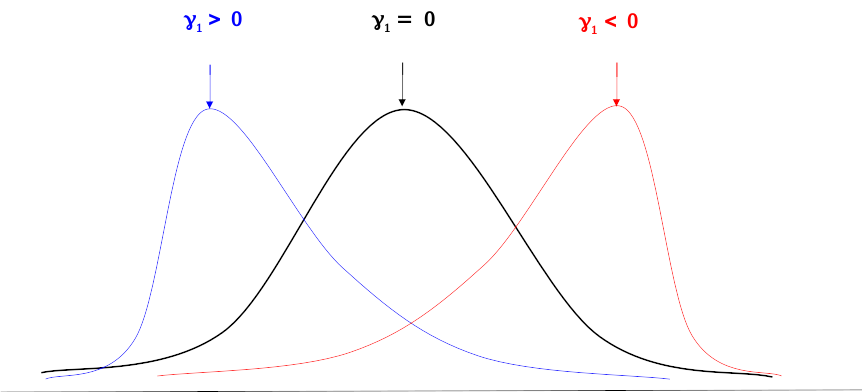
\includegraphics[width=\textwidth]{figures/skewness.png}
    \caption{Šikmosť}
    \label{fig:skewness}
\end{subfigure}
\hfill
\begin{subfigure}[b]{0.48\textwidth}
    \centering
    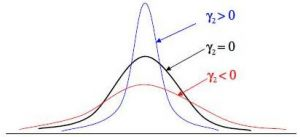
\includegraphics[width=\textwidth]{figures/kurtosis.png}
    \caption{Špicatosť}
    \label{fig:kurtosis}
\end{subfigure}
\caption{Dopad šikmosti a špicatosti na histogram distribúcie}
\end{figure}

Závislosť dvojíc veličín sa vyjadruje \emph{kovariancia} $cov(\mathbf{x}, \mathbf{y})$ a \emph{korelácia} 
$\rho(\mathbf{x}, \mathbf{y})$. U vektora akcelerácie nás bude napríklad zaujímať vzájomná korelácia medzi 
osami pohybu: $\rho(\vec{x},\vec{y}),\, \rho(\vec{x},\vec{z}),\, \rho(\vec{y},\vec{z})$ upozorňujúca na diagonálny 
pohyb alebo podobné budenie v oboch korelovaných smeroch a tým umožňujúce redukciu údajov z dôvodu redundancie.
Kovariancia je daná strednou hodnotou súčinu odchýlky od priemeru zodpovedajúcej premennej (vzťah \ref{eq:covariance}). 
Normovaním kovariancie smerodajnými odchýlkami veličín získame \emph{Pearsonov korelačný koeficient}
(vzťah \ref{eq:correlation}), ktorý je z intervalu $[-1; 1]$.  Hodnota koeficientu $-1$ značí nepriamu lineárnu závislosť
a $+1$ priamu závislosť. 
\begin{ceqn}\begin{align}
\mathrm{cov}(\mathbf{x}, \mathbf{y}) &= \frac{1}{n} \sum_{t=1}^{n}{(x_t - \bar{x})(y_t - \bar{y})} \label{eq:covariance} \\
\rho(\mathbf{x}, \mathbf{y}) &= \frac{\mathrm{cov}(\mathbf{x}, \mathbf{y})}{\sigma_x \sigma_y} \label{eq:correlation}
\end{align}\end{ceqn}

\subsection{Algoritmy na rozpoznávanie špičiek}
\label{peak-detection}
Detekcia udalostí a významných zmien signálového priebehu sa spolieha na hodnovernú identifikáciu špičiek amplitúdy.
Dôležitými indikátormi pre celkovú charakterizáciu javu slúži potom časová pozícia špičky v rámci prúdu, výška prejavujúca
sa získanou úrovňou, šírka obsahujúca údaj o trvaní, či plocha stvárňujúca energiu. 

Ekvivalentne sa špičky z matematického hľadiska stotožňujú s lokálnymi extrémami funkcie, čo sú maximá (vrcholy) a minimá (údolia). 
Podľa definície je lokálne maximum $t_0$ bodom, ktorý má vyššiu funkčnú hodnotu ako všetky ostatné body na intervale 
$t_0 \in I$ (\ref{equ:local-maxima}), lokálne minimum má naopak najnižšiu hodnotu na intervale (\ref{equ:local-minima}) 
\cite{survey-peaks-valleys}. 

\begin{ceqn}\begin{align}
f[t_0] \geq f[t],\, \forall t \in I \label{equ:local-maxima}\\
f[t_0] \leq f[t],\, \forall t \in I \label{equ:local-minima}
\end{align}\end{ceqn}

Kľúčové pre spoľahlivé určenie extrémov je práve interpretácia intervalu $I$ v algoritmoch, ktoré zastupujú rozličné 
potreby korektného vyhodnotenia. Jediné minimum a maximum sa dosiahne zvolením celej dĺžky záznamu za interval, čím sa 
stratia dočasné disturbancie. Na druhej stane prílišným skrátením intervalu sa skoro všetky vzorky budú javiť ako náhle zmeny.

Skutočné signály sa potýkajú so šumom, ktorý sťažuje odlíšenie pravej tendencie od krátkodobých výkyvov. 
Pred samotným procesom hľadania špičiek je preto aplikovaný vyhladzovací filter, v prípade potreby aj opakovane na už
vyhladení signál. Najčastejšie sa jedná o filter 
kĺzavého priemeru, Savitzky–Golay alebo Gaussov filter \cite{spectrometry-peak-detection}. Filtrovanie sa realizuje 
diskrétnou jednorozmernou konvolúciou vstupného signálu a masky filtra $y[n] = x[n] * w[n]$, 
ktorá býva hardvérovo akcelerovaná inštrukciami 
,,fused multiply-add''\footnote{\url{https://developer.arm.com/documentation/102198/0200/Convolution}}.

\subsubsection{Detekcia špičiek prahovou úrovňou}
Za predpokladu, že priebeh meranej veličiny sa vyznačuje krátkymi impulzmi s viac-menej pravidelnou amplitúdou 
je priamočiarou metódou na odlíšenie špičiek od hladín nízkej aktivity určenie prahu $\theta$, ktorý zaregistruje
všetky väčšie hodnoty. Lokálne extrémy sú potom vzorky signálu spĺňajúce podmienku: 
\begin{ceqn}\begin{align}
|f[t]| \geq \theta
\end{align}\end{ceqn}

Určenie takejto hraničnej hladiny prebieha zväčša empiricky alebo na základe heuristík, ktoré so sebou nesú 
domnienku o vlastnostiach priebehu pozorovaní. Uspokojivými odhadom za určitých okolností môžu byť prahy $\theta$: 
viac ako priemer s toleranciou, horné $3/4$ celkového nedávneho rozsahu hodnôt, či dokonca viac ako $k$
smerodajných odchýlok. Odlišné nazeranie na prahovú hodnotu spočíva v jej nastavení pre rozpoznanie 
vzájomnej korelácie signálu a masky zodpovedajúcej tvaru impulzu. Táto úvaha sa opiera o to, že impulz
musí byť dostatočne pravidelný, aby bol nezameniteľne odlíšiteľný.

\subsubsection{Význačnosť vrchola spomedzi susedov}
Doplnkom ku rozpoznávaniu špičiek podľa absolútnej prahovej úrovne je porovnávanie bodov na 
obe strany od preskúmavaného vrchola, čím zistíme relatívnu významnosť extrému pre najbližšie susedstvo.
Aby bola hodnota na danej pozícii $t$ označená za špičku v okolí pozostávajúcom z $k$ priľahlých bodov,
musí byť v porovnaní so všetkými väčšia. Pre okrajové dátové body $f[0]$ a $f[n]$ dochádza k porovnaniu 
iba z jednej strany \cite{survey-peaks-valleys}.
\begin{ceqn}\begin{align}
f[t-i] < f[t] > f[t+i],\quad \forall i \in 1, 2, ..., k
\end{align}\end{ceqn}

Algoritmus č.\ref{algo:neighbours} ,,najvyšší spomedzi susedov'' 
\footnote{\url{https://terpconnect.umd.edu/~toh/spectrum/PeakFindingandMeasurement.htm}} 
prechádza postupne pozorovania veličiny zo zoznamu $y$ a ku kandidátnej špičke na indexe $i$ preveruje najbližších
$k$ hodnôt na obe strany, ak existujú.
\begin{algorithm}[h]
\caption{Najvyšší spomedzi susedov}
\begin{algorithmic}[1]
\Function{Find\_Peaks\_Neighbours}{$y$, $k$, $\varepsilon$, $h_{rel}$, $h$}
	\State $peaks \gets []$ 	\Comment{Zoznam indexov nájdených špičiek v signále $y$}
	\For{$i \gets 0$ \textbf{to} $length(y)$}
		\If {$h \neq null$ \textbf{and} $|y[i]| < h$}  \Comment{Preskoč príliš nízke magnitúdy}
			\State \textbf{continue}
		\EndIf
		\State $possible\_peak \gets true$
		\State $a \gets max(i - k, 0)$
		\State $b \gets min(i + k, length(y))$
		\For{$j \gets a$ \textbf{to} $b$}			\Comment{Porovnaj špičku s bodmi v susedstve}
			\If {$i \neq j$ \textbf{and} $y[j] - y[i] > \epsilon$}
				\State $possible\_peak \gets false$     \Comment{Kopec nie je dostatočne strmý}
			\EndIf
		\EndFor
		\If {$possible\_peak = true$ \textbf{and} $y[i] - \min(y[a], y[b]) > h_{rel}$}
			\State $peaks \gets peaks + [j]$    \Comment{Kandidát je prehlásený za špičku}
		\EndIf
	\EndFor
	\State \Return $peaks$
\EndFunction
\end{algorithmic}
\label{algo:neighbours}
\end{algorithm}
Keď po preskúmaní zostáva $y[i]$ najväčšou hodnotou spomedzi susedov
v rozmedzí $[a; b]$, za tolerancie strmosti stúpania $\varepsilon$ medzi pozorovaniam, a súčasne je relatívna 
výška vrcholu väčšia oproti nižšiemu okraju než nastavený parameter $h_{rel}$ potom je kandidátny bod prehlásený
za skutočnú špičku a pridaný do zoznamu $peaks$. 

Súčasťou algoritmu je tiež preskočenie hodnôt, ktoré nespĺňajú základný predpoklad pre absolútnu amplitúdu $h$. 
Časová zložitosť pre rozhodnutie o jednej špičke je lineárna v závislosti od veľkosti posuvného okna uvažovaného
susedstva $\mathcal{O}(2k)$.

\subsubsection{Algoritmus prechodu nulou do záporu}
Pomyselné vrcholy a údolia v zosnímaných hodnotách sú miestom, kde sa mení smer úrovní amplitúdy zo stúpania na klesanie alebo
z klesania na stúpanie, čím na pomedzí týchto opozitných trendov vzniká stacionárny bod, kde je prvá diferencia nulová: 
$\Delta f[i] = 0$. V lokálnom maxime dochádza súčasne k zmene znamienka prvej diferencie z kladného na záporné. Prudkosť
kopca vyplýva z absolútnej hodnoty diferencie. 

Viacnásobné vyhladenie signálu predom je nesmierne dôležité, 
pretože algoritmus č.\ref{algo:zero-crossing} ,,prechodu nulou do záporu'' (Negative Zero-Crossing) je nesmierne citlivý
na zákmity a nesprávneby ich považoval za špičky. Zvýšenie odolnosti proti takýmto tendenciám sa dosahuje dlhšou sečnicou
spájajúcou bod $i$ s $k$-tou vzorkou vedľa, ktorá sa použije namiesto diferencie s jednotkovým krokom.
\begin{algorithm}[h]
\caption{Prechod prvej derivácie nulou do záporu}
\begin{algorithmic}[1]
\Function{Find\_Peaks\_Zero\_Crossing}{$y$, $k$, $\varepsilon$, $slope$}
	\State $peaks \gets []$
	\For{$i \gets k$ \textbf{to} $length(y) - k$}
		\If {($|y[i+k] - y[i-k]| \leq \epsilon$ \textbf{and} 
		     \State \hskip1.5em $(y[i+k] - y[i]) - (y[i] - y[i-k]) < 0$ \textbf{and}
		     \State \hskip1.5em $|(y[i+k] - y[i]) - (y[i] - y[i-k])| > slope$)}
		    \State $peaks \gets peaks + [i]$
		
		\EndIf
	\EndFor
	\State \Return $peaks$
\EndFunction
\end{algorithmic}
\label{algo:zero-crossing}
\end{algorithm}

Označenie kandidátneho bodu za špičku v zozname hodnôt $y$ stojí na teda troch kritériách. Sklon sečnice sa musí v 
rámci tolerancie $\varepsilon$ blížiť nule, rozdiel prvých diferencií $\Delta y[i+k] - \Delta[i]$ musí byť záporný a veľkosť 
rozdielu diferencií prekračuje prahovú strmosť kopca $slope$, kde leží uvažovaný vrchol. Časová zložitosť
pre jednu špičku je $\mathcal{O}(1)$. 

\begin{figure}[h]
    \centering
    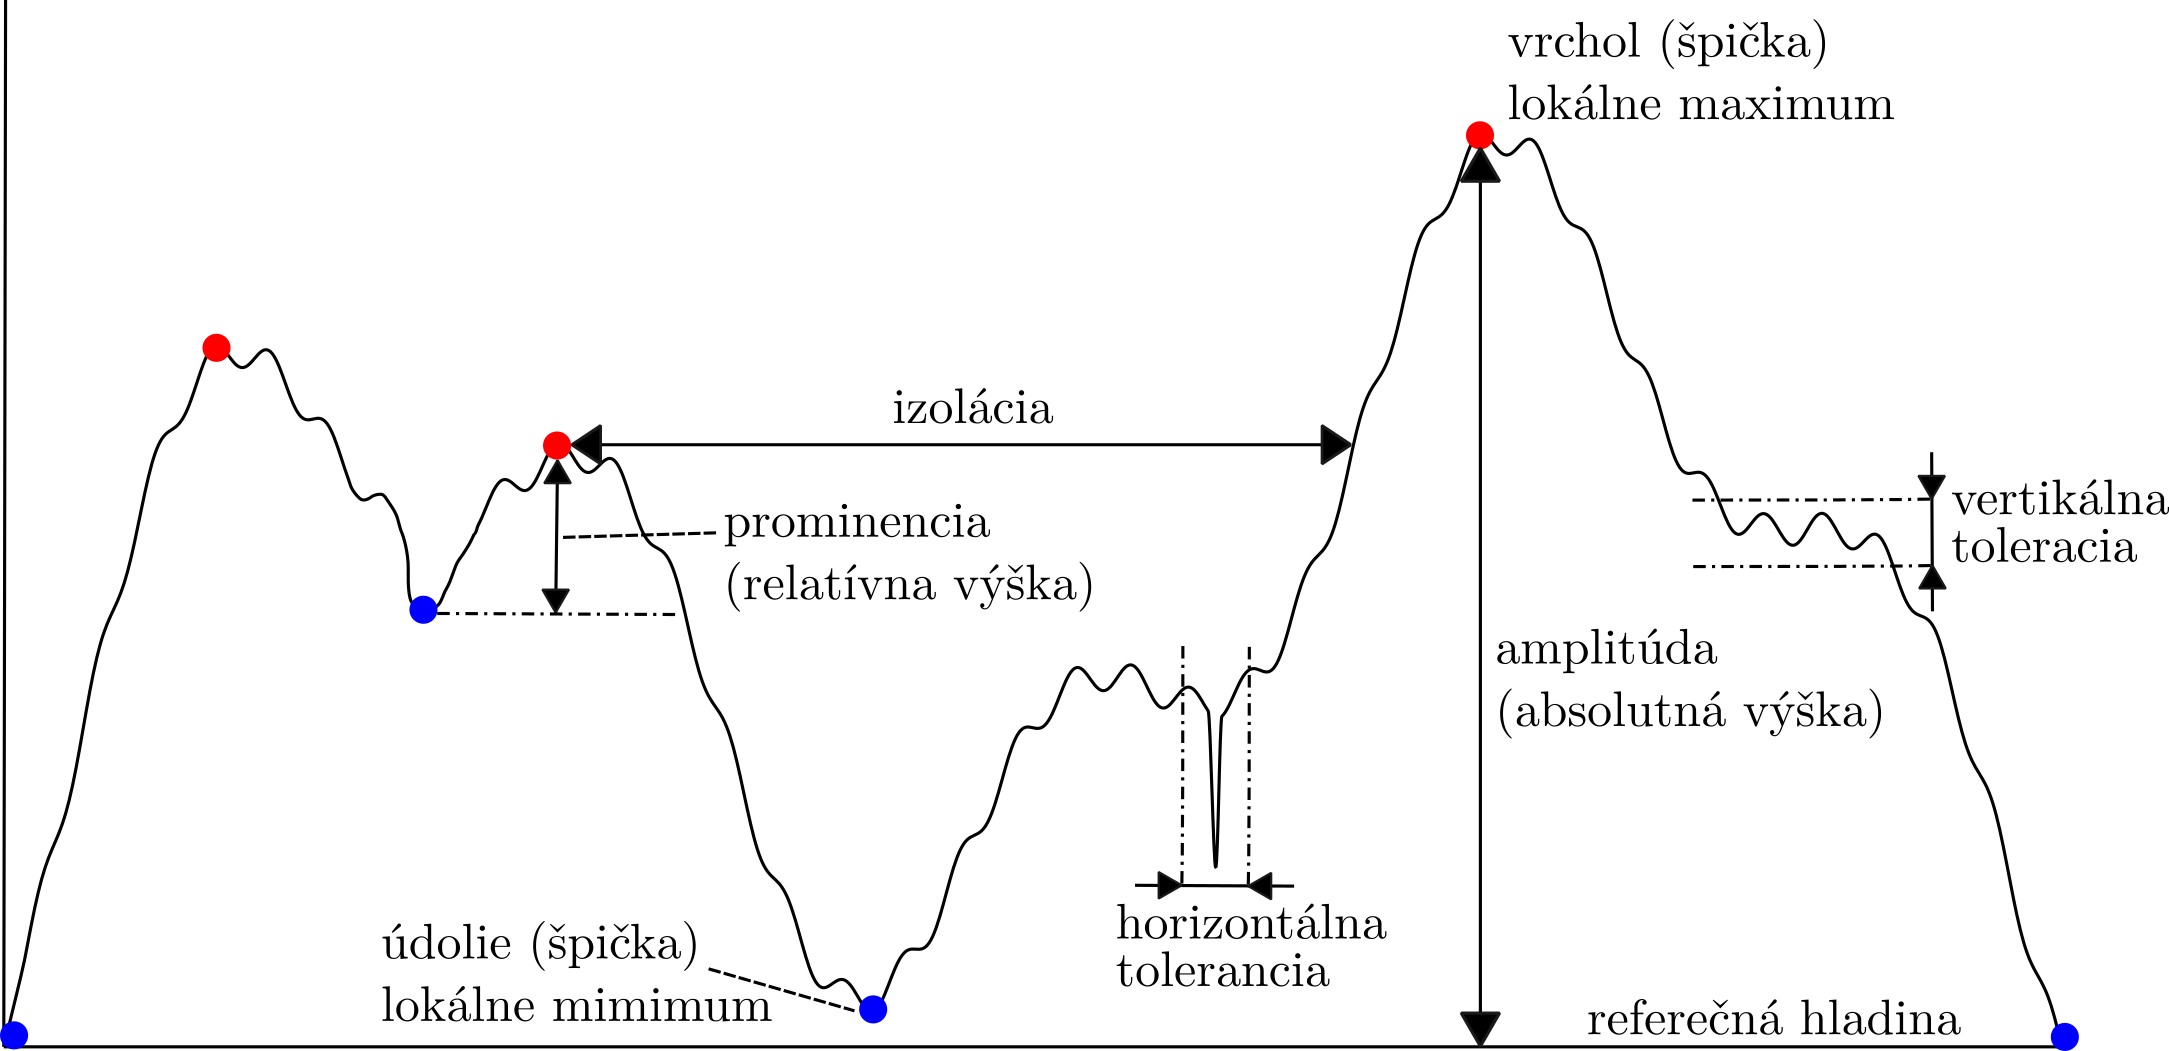
\includegraphics[width=0.9\textwidth]{figures/topography.png}
    \caption{Topografia priebehu signálu}
    \label{fig:topography}
\end{figure}

\subsubsection{Algoritmus horského turistu}
Zanesením do grafu pripomína priebeh funkcie kmitajúceho deja členité pohorie. Na problém rozhodovania sa o tom, či danú lokalitu
považovať za vrchol možno nahliadať z pohľadu chodca cestujúceho po krivke z lineárne interpolovaných vzoriek. V princípe
ide myšlienkou o jednoduchý stavový automat sledujúci aktuálny stav terénu a konajúci rozhodnutia na základe predošlej
skúsenosti v intenciách rozhodovacích pravidiel.

Algoritmus č.\ref{algo:mountain-hiker} horského turistu na začiatku púte z počiatočných bodov zistí, ktorým z dvoch vertikálnych
smerov sa krivka uberá. V prípade, že po druhom kroku dôjde k zmene smeru zapíše sa indikácia možného spádu kopca. 
Výchylka môže byť v dôsledku neprekročenia prahových úrovní v horizontálnej ($hole$) a vertikálnej ($tolerance$) osi 
ignorovaná, lebo ani na lesnom chodníku sa nepovažuje každá jama alebo vydutie za horu. 

Domnelý vrchol je označený za lokálne maximum, keď spĺňa parametre pre topografické vlastnosti minimálnej akceptovateľnej 
prominencie a izolácie (obr. \ref{fig:topography}. Prominencia znamená relatívnu výšku oproti predošlej navštívenej doline. Izolácia vyčísľuje vzdialenosť k najbližšiemu skoršiemu vrcholu. Podobný algoritmus už existuje v literatúre \cite{peek-mountaineer-method}, avšak nižšie prezentovaný pseudokód je oproti nemu zjednodušený a doplnený o požadované tolerancie.
\begin{algorithm}[h]
\caption{Algoritmus horského turistu}
\begin{algorithmic}[1]
\Function{Find\_Peaks\_Hill\_Walker}{$y$, $tolerance$, $hole$, $prominence$, $isolation$}
	\State $peaks \gets []$
	\State $i\_change \gets 0$
	\State $y\_valley \gets 0$
	\State $possible\_change \gets false$
	\State $uphill \gets (y[1] - y[0]) \geq 0$
	
	\For{$i \gets 1$ \textbf{to} $length(y)$}
		\State $y\_step \gets y[i] - y[i-1]$
        \State $slope \gets y\_step \geq 0$

        \If {$possible\_change = false$ \textbf{and} $uphill \neq slope$}
        	\State $possible\_change \gets true$   \Comment{Označenie potenciálneho extrému}
        	\State $i\_change \gets i - 1$
        \ElsIf {$possible\_change = true$ \textbf{and} $uphill = slope$}
        	\State $possible\_change \gets false$  \Comment{Potenciálny extrém bol zachvením}
        \EndIf
        
        \If {($possible\_change = true$
        	\State \hskip1.5em \textbf{and} $uphill \neq slope$
        	\State \hskip1.5em \textbf{and} $|i - i\_change| > hole$
        	\State \hskip1.5em \textbf{and} $|y[i] - y[i\_change]| > tolerance$)}

        	\State $posible\_change \gets False$        \Comment{Významný lokálny extrém potvrdený}
        	\State $prev\_uphill \gets uphill$
        	\State $uphill \gets slope$
        	
        	\If {$prev\_uphill = false$ \textbf{and} $uphill = true$}
				\State $y\_valley \gets y[i\_change]$   \Comment{Nájdené údolie}
                
            \ElsIf {($prev\_uphill = true$ 
            		\State \hskip1.5em \textbf{and} $uphill = false$
            		\State \hskip1.5em \textbf{and}  $|y[i - hole] - y\_valley| > prominence$)
            		\State \hskip1.5em \textbf{and}  $|y[i - hole] - y[last(peaks)]| > isolation$)}
				\State $y\_peak \gets y[i\_change]$    \Comment{Skutočný vrchol identifikovaný}
				\State $peaks \gets peaks + [i_change]$              
            \EndIf      	
        \EndIf       
	\EndFor
	\State \Return $peaks$
\EndFunction
\end{algorithmic}
\label{algo:mountain-hiker}
\end{algorithm}
\afterpage{\clearpage}

\subsection{Metriky pre binárny klasifikátor}
Uviedli sme tri rozdielne rovnocenné prístupy odhalenia špičiek uplatniteľné v nasadení online na sústavný prúd údajov
separovaný do blokov posuvným oknom. Rozobrali sme algoritmus opierajúci sa o porovnávanie striktne usporiadaných 
susedov na obe stany, algoritmus využívajúci sklon sečníc vychádzajúc s vlastností prvej derivácie a napokon
stavový automat odvolávajúci sa na sekvenčne preskúmavanú topografiu krivky grafu. Spoločným rysom zmienených techník 
je vykonávanie binárne zaradenie pre každú vzorku, či sa sa nachádza alebo nenachádza na aktuálnej pozícií vrchol.

Rozhodnutie môže viesť k správnemu $P$ alebo nesprávnemu $N$ riešeniu vzhľadom na objektívnu pravdu 
sprostredkovanú anotovanými dátami. Keď sa kategorizácia zhoduje s realitou dostávame skupiny 
skutočne pozitívnych $TP$ a skutočne negatívnych $TN$. V prípade, že sa klasifikátor pomýli vyjde buď chyba
prvého rádu $FP$, kedy registrujeme neexistujúcu špičku, alebo chyba druhého rádu $FN$, kedy ju prehliadneme.
Umiestnením počtov charakteru rozhodnutí do tabuľky vzniká matica zámen.

Úspešnosť klasifikačných algoritmov pre ich vzájomné porovnanie kvantifikujú viaceré metriky. Na odladenie parametrov 
vplývajúcich na náchylnosť preferovať kladné alebo záporné výsledky sa vzťahuje \emph{prevalencia} výskytu očakávaného
javu: $P / (P+N)$ v samotných dátach. Snahou rozhodovania je maximalizovať senzitivitu a špecifickosť výsledkov algoritmu. 
\emph{Senzitivita} (\ref{equ:sensitivity}) udáva koľko bodov, ktoré sú prehlásené za špičky naozaj je špičkami. 
\emph{Špecifickosť} (\ref{equ:specifity}) sa zameriava na potvrdenie, aké množstvo pozorovaní nepovažovaných za špičky,
nie sú nimi aj skutočne. 
\begin{ceqn}\begin{align}
TPR = \frac{TP}{P} = \frac{TP}{TP + FN} \label{equ:sensitivity} \\
TNR = \frac{TN}{N} = \frac{TN}{TN + FP} \label{equ:specifity}
\end{align}\end{ceqn}

Presnosť určenia lokálneho extrému sa skladá z správnosti (\ref{equ:ppv}) a precíznosti (\ref{equ:accuracy}),
ktoré je rovnako žiaduce dosahovať čo najbližšie sto percentám, pri nízkej chybovosti (\ref{equ:error-rate}), čiže
nízkeho počtu falošných poplachov.
\begin{ceqn}\begin{align}
PPV = \frac{TP}{TP + FP} \label{equ:ppv} \\
ACC = \frac{TP + TN}{P + N}\label{equ:accuracy} \\
FPR = \frac{FP}{FP + TN} \label{equ:error-rate}
\end{align}\end{ceqn}

Štandardným nástrojom na vyjadrenie kvality binárneho klasifikátora je \emph{ROC krivka} zakresľujúca 
senzitivitu $TPR$ vo zvislom smere voči vodorovnej chybovosti $FPR$. ROC vytvoríme graduálnym posúvaním prahu 
pre klasifikáciu prostredníctvom parametrov algoritmu. Použiteľný algoritmus sa vyznačuje vypuklou krivkou
smerom k ľavému hornému rohu nad diagonálou, ktorá by sprevádzala počínanie náhodného rozhodovania. Dokonalá
metóda pri dosahovala stopercentnú senzitivitu za nulovej chyby. Vyjadrením plochy pod ROC krivkou je miera AUC,
ktorá umožňuje približné číselné porovnanie rôznych získaných kriviek.

\section{Frekvenčná a časovo-frekvenčná analýza signálu}
Vibrácie prítomné v získanom zázname zrýchlenia sa prejavujú s variabilnou pravidelnosťou a cyklickým opakovaním, ktoré
vyplýva z povahy monitorovaného pohybu.

\cite{time-series-analysis}
vlastnosti frekvenčného spektra,
decibele, 
spektrogram,
odstup od šumu (SNR),
power spectrum density (dbFS),
spektrálny analyzátor

\subsection{Fourierová transformácia}
Diskrétna fourierová transformácia mapuje signál dĺžky $N$ do množiny $N$ diskrétnych frekvenčných komponentov. \cite{signal-processing}
\begin{equation}
X = \mathbf{W}x; W_{nk} = e^{-i\frac{2\pi}{N}nk} = W_N^{nk}
\end{equation}
Inverzná transformácia
\begin{equation}
x = \frac{1}{N}\mathbf{W}^H X
\end{equation}

Integrálne transformácie: Fourierová transformácia (CFT, DFT), Kosínusová transfomácia (MDCT), \cite{dct} 
\cite{casove-frekvencia-analyza-signalu}

\begin{ceqn}\begin{align}
\mathcal{F}: X(\omega) = \int_{-\infty}^{+\infty}{x(t) \cdot e^{-i\omega t} \mathrm{dt}}
\end{align}\end{ceqn}

\subsection{Algoritmus FFT pre DFT a DCT}
Opis DIT radix-2 FFT algoritmus komplexných, reálny, pre MDCT \cite{fft-blackbox}
konštantný digitalizačný krok bez prerušení a navyše dĺžka radu musí byť celočíselná mocnina dvoch (s.29)

prevádza konečnú sekvenciu dát na súčet kosínov oscilujúcich na rôznych frekvenciách

\begin{ceqn}\begin{align}
X[m] &= \sum_{n = 0}^{N-1}{x[n] \cdot e^{-i2\pi n m / N}} \\
X[m] &= \sum_{n = 0}^{N-1}{x[n] \cdot [\cos(2\pi n m / N) - i \cdot \sin(2\pi n m / N)]}
\end{align}\end{ceqn}

Frekvenčné rozlíšenie
\begin{equation}
\Delta f = \frac{f_s}{N}
\end{equation}

$$X_{k}=\sum_{n=0}^{N-1} x_{n}\cos \left[\,{\frac{\pi}{N}}\left(n+{\frac{1}{2}}\right)k\right]\qquad \,
k=0,\ \dots \ N-1 $$
$$X_{k}=\sum _{n=0}^{N-1}x_{n}\cos \left[\,{frac{\pi}{N}}\,\left(n+{1}/{2}\right)\left(k+{1}/{2}\right)\right]\qquad
\,k=0,\ \ldots \ N-1$$
$$X_{k}=\sum _{n=0}^{2N-1}x_{n}\cos \left[{\frac {\pi }{N}}\left(n+{\frac {1}{2}}+{\frac {N}{2}}\right)\left(k+{\frac {1}{2}}\right)\right]$$

\subsection{Oknové funkcie}
the DFT implicitly assumes that the signal is periodic, i.e. that the time series of length N repeats itself
infinitely in a cyclic manner.  If the frequency of the sinusoidal input
signal is not an exact multiple of the frequency resolution fres , i.e. does not fall in the exact
center of a frequency bin, this assumption is not true, and the DFT will ‘see’ a discontinuity
between the last sample and the first sample due to the cyclic continuation. That discontinuity
spreads power all across the spectrum. \cite{spectral-density-estimation}

Pri FT dostávame frekvenčné zložky za prítomné v celkom priebehu v rôznych časových okamihoch, keby sme chceli
dosiahnuť lepšiu lokalizáciu v čase, tak prvý pokus ponúka Gáborova transformácia. Princíp neurčitosti: sústredenosť 
vo frekvenčnej domény vyvoláva neurčitosť v čase a symetricky naopak.

Dochádza k vynásobenie zdrojového signálu koeficientmi okna pre odstránenie hraničných efektov, ktoré spôsobujú/vnášajú
neexistujúce periodické komponenty, na okraji okna preto znižuje úroveň na nulu. Snahou je dokonalé izolovanie frekvenčného
pásma, ale pri FT dostávame sinc.
Prehľad okien - symetrické okolo stredu

\begin{ceqn}\begin{align}
\text{Obdĺžníkové (rovnomerné) okno} w(n) &= 1,\, n = 0, 1, ..., N - 1 \\
\text{Trojuholníkové (Barlett) okno} 
	w(n) &= 
	\begin{cases} 
		\frac{n}{N / 2}; n = 0, \dots, N / 2 \\
	 	2 - \frac{n}{N / 2}; n = N/2+1, \dots, N - 1  
	\end{cases} \\
\text{Hanningovo okno} w(n) &= 0.5 - 0.5\cos(2\pi n / N)  \\
\text{Hammingovo okno} w(n) &= 0.54 - 0.46\cos(2\pi n / N) \\
\text{Blackman-Harrisovo okno} w(n) &= 0.35875 - 0.48829\cos(z) + 0.14128 cos(2z) - 0.01168 cos(3z), z = 2\pi n / N
\end{align}\end{ceqn}

Efekt oknových funkcií na spektrálny leakage efekt (únik spektra)
výhodné percentá prekryvu FT 	\cite{understanding-dsp} \cite{spectral-density-estimation}
Priemerovanie a prekryv:
- Amplitude Flatness (AF)
- Power Flatness (PF)
- Overlap Correlation (OC)

\subsection{Filtre s konečnou impulznou odozvou}
\label{fir-filter}
Roziel medzi FIR a IIR, Dolná pripusť, pásmová priepusť, horná pripusť,
 Konvolúcia a konvolučné jadro, konvolučná veta, účel: identifikácia prítomnosti známej frekvencie v signále akcelerácie
\begin{equation}
y(n) = \sum_{k=0}^{D_y}{x(k) \cdot h(n-k)} = x(n) * h(n)
\end{equation}
Prenosová funkcia - koeficienty filtra

\subsubsection{Detektor obálok}
\footnote{\url{https://www.mathworks.com/help/dsp/ug/envelope-detection.html}}
\footnote{\url{https://www.dsprelated.com/showarticle/938.php}}
- Square-Law / Full-Wave
- umocnenie dvomi  (alebo absolútna hodnota)
- amplifikácia faktorom 2 (zostane iba horná polovica)
- decimácia 1.5 (podvzorkovanie)
- dolná priepusť FIR
- druhá odmocnina pre odstránenie skreslenia spôsobeného úvodným umocnením
- 

\section{Senzorová sieť}
Nízko-energetické zariadenia komunikujúce cez odľahčené sieťové protokoly so snahou spracovania v reálnom čase a ponechaním najdôležitejších informácii dolovaním z veľkého množstva zdrojových dát. Cloud / Hmlové počítanie. okrajový a sink (zoskupujúci) uzol

Vlastnosti senzorovej siete
\begin{itemize}
\itemsep0em
\item Autokonfigurácia senzora - reakcia na zmeny v sieti a prostredia pôsobenia
\item Škálovateľnosť - veľké množstvo senzorov so spoločným účelom a schopnosťou vzájomnej kooperácie a interoperability.
\item Odolnosť voči chybám - v prípade pridania alebo odobratia uzla budú spojenia bez prerušenia.
\item Energeticky efektívna komunikácia uzlov - s upravenými protokolmi štandardného sieťového zásobníka
\begin{itemize}
\itemsep0em
\item Event-driven - stály zber dát a reakcia na náhle zmeny. posielajú údaje až po prekročený kritického prahu
\item Query-driven - zbierajú údaje iba po prijatí dopytu od používateľa
\item Time-driven - pravidelne odosielajú údaje sinku. vzorkovaciu frekvenciu volí sink
\end{itemize}
\end{itemize}
\cite{wsn-overview}

Spracovanie toku informácií (IFP - Information flow processing) - nástroj na včasné spracovanie dát ako tečie z periférií do centra systému. Snahou je ukladanie agregovaných štatistík, napr. detektor požiaru za použitia čidiel teploty a dymu nepotrebuje ukladať jednotlivé merania, lebo sú samo o sebe nepodstatné. Keď nastane varovná situácia, je potrebné aby tá obsahoval všetky údaje na lokalizáciu ohniska.

CEP - Complex event processing - spracúva toky udalosti zo zdrojov reálneho sveta na základe aplikovania aktívnych pravidiel stanovených správcami systému a poupraví toky do komplexnejšieho výstupu. Pravidlá sú v tvare Event-Condition-Action (ECA).
\begin{itemize}
\itemsep0em
\item Udalosť - definuje zdroje ako generátory udalostí
\item Podmienka - uvažuje ktorá časť udalosti bude braná do úvahy pri spracovaní, napr. môže ísť o prekročenie prahu
\item Akcia - aká sada úloh má byť vykonaná pri detekcii udalosti
\end{itemize}
\cite{processing-information-flows}

Súčasti senzorovej jednotky: Zberná jednotka, Výpočtová jednotka, Komunikačná jednotka, Napájacia jednotka

Obmedzenia na senzorové uzly
\begin{itemize}
\item Spotreba energie - energetická autonómia uzlov vo WSN umožňuje nasadzovanie zariadení do odľahlých miest pre využitie v inteligentných mestách alebo na účely ochrany prírody. životnosť senzorovej jednotky je ohraničená kapacitou batérie.
\item Dosah komunikácie - Senzory disponujú obmedzenou energiou na vysielanie a dosah je negatívne ovplyvnený silou signálu na anténe. Z toho vyplývajú aj nižšie prenosové rýchlosti.
\item Výpočtový výkon a úložisko - Nízka taktovacia frekvencia procesora v megaherzoch a veľkosti pracovných pamätí v stovkách kilobajoch alebo megabajtoch.
\end{itemize}
\cite{big-data-collection-wsn}

Bluetooth, BLE -  IEEE 802.15.1 bezdrôtová technológia s krátkym dosahom spravidla do 10 m (0,5mW pri 0.5m, 1mW pri 1m, 2.5mW pre 10m, 10mW pre 20m) na ultra krátkych vlnách 2.402 GHz - 2.48 GHz.
SDP, RFCOMM náhradou za sériové porty + L2CAP. (symetrická komunikácia) \url{https://www.bluetooth.com/specifications/specs/rfcomm-1-2/}
Wifi - 802.11 (klient-server cez prístupový bod) - TCP/IP sieťový zásobník, CoAP, MQTT na 6LoWPAN 
LoRa 863-870Hz
IEEE802.15.4e (Smart Mesh IP)  Time Synchronized Mesh Protocol (TSMP) The TSMP includes a Time Slotted Channel Hopping (TSCH) media access layer (MAC). TSCH works by dividing time into ‘slots’, and providing a mechanism to map time slots to channels with a pre-assigned hopping sequence.
Zigbee

